\documentclass[11pt]{article}
\usepackage[margin=1in]{geometry}
\usepackage[utf8]{inputenc}
\usepackage{ulem}
\usepackage{xcolor}
\usepackage{natbib}
\RequirePackage[framemethod=tikz]{mdframed}

\usepackage{graphicx}
\usepackage[affil-it]{authblk}

% paragraph formatting
\setlength{\parindent}{0em}
\setlength{\parskip}{0.5em}
\renewcommand{\baselinestretch}{1.5}

\newcommand{\rw}[1]{{\textcolor{red}{[RW: #1]}}} % %RW comment
\newcommand{\edit}[1]{{\textcolor{red}{#1}}} % %edit
\definecolor{armygreen}{rgb}{0.29, 0.33, 0.13}
\newcommand{\aw}[1]{{\textcolor{armygreen}{[AW: #1]}}} % %AW comment

\newenvironment{boxedtext}[1]{%
  \begin{mdframed}[frametitle=#1,
    frametitlefont=\scshape\mdseries\sffamily,
    frametitlealignment=\centering,
    backgroundcolor=black!20,
    hidealllines=true,
    innerleftmargin=11\p@,innerrightmargin=11\p@,
    frametitleaboveskip=0.5\baselineskip,
    innerbottommargin=0.5\baselineskip,
    skipabove=\baselineskip,skipbelow=0.5\baselineskip]
}{%
  \end{mdframed}%
}


\title{Understanding the tripartite approach to Bayesian divergence time estimation}
\author[1,2]{Rachel C. M.  Warnock} \author[3]{April M. Wright}
%alphabetical for the time being

\affil[1]{Department of Biosystems Science and Engineering, ETH Z\"urich, Basel, Switzerland}
\affil[2]{Swiss Institute of Bioinformatics (SIB), Switzerland}
\affil[3]{Department of Biological Sciences, Southeastern Louisiana University, Hammond, United States}

\date{}

\begin{document}

\maketitle

\section{Abstract}

Placing evolutionary events in the context of geological time is a fundamental goal in  paleobiology and macroevolution.
In this article we describe the tripartite model used for Bayesian estimation of time calibrated phylogenetic trees.
The model can be readily separated into its component models: the substitution model, the clock model and the tree model.
We provide an overview of the most widely used models for each component and highlight the advantages of implementing the tripartite model within a Bayesian framework.

\section{Introduction}

Phylogenetic inference is common in all facets of biology and estimating a phylogeny is a critical step in many comparative analyses. The fact that tree inference is common can obscure the underlying complexity of the task.
When a researcher estimates a phylogeny, they are attempting to reconstruct evolutionary events that potentially occurred millions of years ago.
In modern phylogenetics, generating trees is often achieved using an evolutionary model, which ideally captures the generating processes that underlie our data.
Since no two datasets are exactly the same, in terms of evolutionary history or sampling, 
%, the forces that generated them
%It is therefore important that researchers understand both the data and evolutionary models that allow us to make phylogenetic inferences.
choosing the best approach to build a phylogeny requires deep knowledge of the taxonomic group, as well as phylogenetic theory.
In this review we focus on the models commonly used to infer phylogenies in macroevolution and paleobiology research.

The primary source of evidence used to infer evolutionary relationships are phylogenetic characters: molecular sequences in the case of living species or morphology in the case of most fossils. 
The number of differences observed between samples are used to measure evolutionary distance and to group species together in the tree.
This estimation becomes more challenging if we also need to estimate dated phylogenies.
This is because phylogenetic characters only contain information about \textit{relative} time. 
Additional temporal evidence is required to calibrate trees to \textit{absolute} time.
Otherwise it is not straightforward to distinguish between rapid evolutionary rates over short intervals versus slow evolutionary rates over long intervals.
Fig. \ref{fig:undated} provides a recap of the most important features of a phylogeny (tips, nodes and branches, which together comprise the topology) and shows an example of the output generated by undated and dated phylogenetic inferences. 
An undated phylogeny will typically have branch lengths in units that reflect the overall number of molecular or morphological character changes, while a dated tree will have branch lengths in units of calendar time, such as years or millions of years.

Inferring time calibrated trees is often achieved through jointly estimating the topology and node ages.
In performing this analysis, researchers usually assume a tripartite model of evolution: one model that describes the accumulation of differences in character data, one that describes the distribution of evolutionary rates across the tree, and a model describing the distribution of speciation events (node ages) across the tree \cite{Thorne1998,Kishino2001,Yang2006,Drummond2006}.
This tripartite approach is a product of the history of phylogenetic model development and reflects the way in which researchers have traditionally tried to break down the problem of estimating evolutionary time from phylogenetic character data.
While the tripartite model may sound complex, it enables researchers to treat each component as a discrete inferential module and provides them with the flexibility to combine different models that best suit their data.
Understanding the tripartite framework is therefore useful for tracing the history of model development, making informed parameter choices, interpreting your results and diagnosing problems with your analysis.

We describe the components of the tripartite model in more detail and the processes they aim to capture.
We describe how to perform this analysis using Bayesian methods and highlight some of the advantages of using this statistical framework.
%Bayesian methods have well-developed tools for testing the fit of model assumptions to our data.
%Bayesian approaches allow us to make a wide range of assumptions, and to test how well those assumptions fit the data we have observed.
Finally, we discuss how different aspects of the tripartite model can be linked and how this can be used to test hypotheses in paleobiology.


\section{A brief introduction to Bayesian Inference in phylogeny}

In this review, we focus on divergence time estimation using Bayesian methods. 
These are methods which incorporate prior information and researcher intuition about parameters in our model.
Unlike some other methods, Bayesian methods estimate a sample of phylogenetic trees and values for the parameters of the underlying phylogenetic model.
We can think of Bayesian inference as having three important components: the likelihood, the prior, and the posterior.
Fig. \ref{fig:bayes} provides an overview of how these components are connected via Bayes' theorem to data and the tripartite model of evolution described in this review. %RW: not sure this is the best place to cite this figure %aw{I think it is one of many good places, but yes, it may not be the best first citation ... }

We will be discussing these methods in a Bayesian context for a few reasons.
Perhaps the most important is that Bayesian methods estimate a sample of plausible parameter values under a model. 
A Bayesian method inherently provides an indication of the uncertainty associated with any model parameter.
Since we are unlikely to be able to observe the true parameter values for an event that occurred millions of years in the past, it is prudent to consider possible ranges for parameters in our model.
Bayesian methods also allow researchers to constrain the values an individual parameter can take. 
This is a desirable property because we may have prior information from studies conducted by others about the numerical value of a parameter.
In this way, Bayesian inference provides an intuitive approach to accommodating uncertainty in other evolutionary and sampling parameters, and incorporating our existing knowledge of parameter values.
On a practical level, much of the widely-used divergence time estimation software has been written in a Bayesian context.

%\rw{LH said she didn't think of divergence time estimation and time scaling as interchangeable but I actually do. Now that you've eliminated the term time scaling maybe this doesn't matter?}
%\aw{The more I think about it, the more I don't. I think if we say Bayesian time-scaling, I think of that as interchangeable with divergence time estimation. But coming from a molecular perspective, I also think of things like r8s (which I guess is sort of like some of the post-hoc time scalers you see in paleo) that are really philosophically different than what we're doing here.}
%\rw{Maybe we can leave this until a reviewer/someone else brings it up.}
%aw{Yes, I don't think this is crucial. We can say dated and call it good.}

\subsection{The Likelihood}

We often think of statistical words in colloquial terms.
For instance, we may think of ``likelihood" in our daily life, as an event being likely or unlikely. 
This is different than in a statistics, when we calculate the likelihood, or probability, of observed data given a particular model.
A model is a mathematical description of a phenomenon.
Models are made up of parameters, which are thought to represent key factors of that phenomenon.
The relationship between parameters is described through mathematical expressions.
Many parameters of a model are treated as \textit{random variables}.
A random variable has an unknown value, for which candidate values will be tested as the tree search proceeds. 
In a Bayesian analysis, different values will be \textit{sampled}, or proposed, for each random variable from the range of potential values.
A sample of solutions will be generated, and will be evaluated via both the model and the priors.
In the tripartite model for divergence time estimation, all parts of the model (site model, clock model and tree model) will be represented in the likelihood as well as in the prior (Fig. \ref{fig:bayes}).


\subsection{The Prior}

%\rw{To do: as per DB's suggestion look into Alfaro and Holder's 2006 perspective on priors.}

Bayesian methods incorporate researchers' prior knowledge and beliefs about the values a parameter may take through the use of priors.
A prior specifies a probability distribution from which the value of a particular parameter may be drawn.
A prior distribution should reflect the belief or knowledge a researcher has about the value of a parameter.

Importantly, the value of a parameter can fall outside the prior distribution.
Priors can be enforced with varying degrees of strength.
If the data strongly support a value for a parameter that is in conflict with the prior specified, that value can still be supported if the prior isn't strongly enforced.
Priors can also be chosen to offer maximal flexibility in the potential values for the parameter.
For example, a weak intuition about the value of a parameter can be incorporated via a vague prior.
In biology, it is fairly common to see distributions such as the Gamma or Exponential, which can be very flexible, depending on the centrality and/or shape parameters.

Sometimes the distinction between what we call a model and the prior can be difficult to see (See Box `The Likelihood' for more information.).
By constraining the values a parameter can take, it is possible to steer estimation towards or away from certain sets of values, without changing what facets of the generating process are being modeled. 

\subsection{The Posterior}

The posterior is the outcome of a Bayesian analysis and includes a distribution of plausible for all of the variable parameters in our models, including the topology and divergence times.
This component effectively combines the information from the prior with the likelihood. % \rw{DB doesn't think this is a complete enough description of the posterior.} \aw{It seems good to me?}

Values for each parameter will appear in the posterior distribution in proportion to how probable they are, given our model and priors.
The highest point or points of the distribution represents the most probable parameter estimates.
The variance of the posterior distribution for a given parameter reflects the uncertainty in that estimate.
If the variance in our posterior distribution is relatively high this reflects lots of uncertainty in our parameter estimate.
Conversely, if the variance is relatively low, this reflects low uncertainty in our estimate.
Note that low uncertainty does not necessarily mean a value is true, just that there is high support for it given the data and model.
Similarly, high variance or uncertainty in the posterior does not necessarily mean that the model is incorrect or that the analysis bad. It simply means that there is limited information in our data.
It is also possible to have more than one peak in your posterior sample.
This indicates that multiple solutions are feasible given the model and the data.

From the posterior distribution of many standard model parameters (e.g. rate parameters) we can construct credible intervals, which are the Bayesian equivalent of confidence intervals.  
We typically use the 95\% highest posterior density (HDP) interval, which is the spread of posterior values that contains 95\% of the posterior.
The upper and lower limits of the of 95\% HPD are intuitive way of communicating the uncertainty associated with parameters such as rates or node ages.
Summarizing a posterior distribution of trees is altogether more tricky.
There are a variety of approaches to generating summary trees, which use different strategies for capturing the phylogenetic relationships that are best supported by the posterior.
Support values for each node are typically based on the proportion of trees in the posterior in which that node also appears. 
This is referred to as the posterior probability. 

All approaches to producing summaries of the posterior have benefits and downsides, especially when there is high uncertainty associated with the tree topology.
We emphasise that the posterior output of Bayesian phylogenetic tree inference is really a distribution of trees and associated model parameters. 
We should be careful to avoid placing too much confidence in any one statistic or summary value from that distribution.
Instead, it is important to understand the underlying models used to generate your tree, and how these may result in uncertainty given the data you have.



\section{A tripartite model for divergence time estimation}
 
A model provides us with an expression for calculating the probability of observing our data, given some underlying assumptions about the processes that generated the data. 
%The model will include parameters thought to represent key aspects of these processes.
Perhaps the most obvious thing we need to describe is the process of phylogenetic character evolution.
This is achieved using the \textit{substitution model}, which describes the probability of changing between different character states.
Substitution models are at the core of undated phylogenetic inference and essentially provide a measure of evolutionary distance.
We tend to measure evolutionary distance or branch lengths in an undated phylogeny as the \textit{number of expected substitutions per character}. We use ``expected'' substitutions because models allow for hidden state changes, such that the number of changes could be larger than the number we observe from our data.
As noted above, phylogenetic characters do not contain information about absolute time. Evolutionary distances estimated using the substitution model actually represent a product of rate and time.
Ultimately, we need to be able to estimate the substitution rate in \textit{expected substitutions per character per calendar unit time}.

To extract information about rates and times from phylogenetic character data we need a modeling framework that describes the  relationship between these variables, in addition to the substitution model.
This is achieved with the addition of the two key model components required to date a phylogeny: the \textit{clock model} and the \textit{tree model}.
The clock model describes how the substitution rate varies (or does not) across the tree.
The tree model describes the process of speciation, extinction, and lineage sampling that generated the tree.
To tease apart rate and time we either need to know the average substitution rate or we need to calibrate the substitution rate using temporal information from elsewhere.
For macroevolutionary timescales calibration information typically comes from fossil sampling times or the age of biogeographic events. This information is incorporated into the tree model.
The tripartite approach to divergence time estimation is a hierarchical Bayesian model, which means it links together different sub-models (i.e. the substitution, clock and tree models) (see box).

Note that rate and time are often only semi-identifiable, meaning multiple combinations of parameters can potentially generate the same probability of the observed data.
In this case, we may be unable to identify, or distinguish, the true parameter values.
In practice, this means we need to put strong prior information on the average substitution rate and speciation times. 
A consequence of this that the results will be very sensitive to these priors.
It is important for biologists to understand each of the component pieces (the substitution, clock and tree models) in order to make good parameter choices.

\section{Substitution models}

The first component of the tripartite model is the substitution model.
The substitution model, sometimes called the site model, describes how phylogenetic characters in the dataset evolve.
These models are called substitution models because they were initially written to describe nucleotide changes.
These models describe how character change accumulates over time, leading to the observed phylogenetic data.
In the context of divergence time estimation, phylogenetic data are typically either morphological or molecular data. 
While molecular and morphological data have very different properties, as will be discussed below, similar methods have historically been used to infer phylogeny from them.

Most data used in phylogenetic estimation has been discrete data.
Discrete data can be broken into non-overlapping categories.
For example, nucleotide sequence data separates cleanly into adenine, cytosine, guanine, and thymine.
Morphological characters are often divided into discrete states \cite{de1985ontogenetic}.
Most simply, these may correspond to an absence state (usually coded as `0') and a presence state (usually coded as `1') \cite{watrous1981}.
They may also correspond to more complex character diagnoses.

There are many models to describe how molecular sequence data evolve over time \cite{Jukes1969, Kimura1980, Felsenstein1981, Hasegawa1985, Tavare1986}.
Nucleotide data tend to have well-defined and discrete properties.
This allows a range of assumptions to be made about what changes we are likely to see over evolutionary time.
In most common substitution models, the probability of observing a change from one character state to another is taken to be the product of the \textit{exchangeability} between the two nucleotides at \textit{equilibrium frequency} of the starting nucleotide (i.e., the nucleotide that exists in the sequence, and will be substituted for another). 
The exchangeabilities refer to the probability of seeing a change from one particular state to another.
These are often based on biochemical features of the nucleotide base.
For example, it is unlikely to see a purine (two-ringed nucleotides, adenine and guanine) substituted for a pyrimidine (one-ringed bases, cytosine and thymine). 
This is biochemical --- we are less likely to observe large changes, such as gaining a second ring of carbons on a structure, than we are smaller ones.
Equilibrium frequencies refer to the frequency that we would see each of our character states if we allowed the evolutionary process to run infinitely long (i.e., to equilibrate).
This is based in simple statistics: Even if it is easy to change from one nucleotide to another, if the starting nucleotide is rare, that change will be seldom observed.
It may be easy to transition from an adenine to a guanine.
But if we have no adenines in our dataset, we are unlikely to observe this change over time.
\clearpage












Making different combinations of assumptions can yield a panoply of molecular models.
The simplest model of sequence evolution, the Jukes-Cantor model \cite{Jukes1969}, assumes only one parameter: the rate of evolution.
The exchangeabilities of this model are equal between all states. 
The equilibrium frequencies are also assumed to be equal.
Therefore, under this model, you are as likely to observe a change that adds a second carbon ring to a pyrimidine as you are to observe changes from pyrimidines to other pyrimidines.
On the opposite end of the spectrum, the general time reversible model (GTR) \cite{Tavare1986} allows for six different exchangeabilities, and for each molecular character to have its own equilibrium frequency.
This is a more complex model, but it is often supported as being the correct one for many datasets \cite{abadi2019}.


Bayesian phylogenetics using morphological characters have
historically used a more restricted set of models than analyses of molecular data.
While we may be able to divide a morphological character into multiple states, we may not be able to easily describe how states can transition from one to another over evolutionary time.
Molecular models assume that the biochemical properties of an adenine are the same today as they were in the past, and
that all adenines are the same in different locations in the dataset.
What are the biochemical properties of an absent character?
Does a change from `0' to `1' at character `1' imply the same magnitude of changes as the same change at character `5'?
The lack of consistent meanings to character states has limited the assumptions that can be made about the process that generated morphological data.
Due to the limited number of morphological models available, model testing has not become common in morphological phylogenetics yet (though see an example of empirical model fitting in \cite*{bapst2017}), and understanding the role of the morphological model in divergence time estimation is an active area of scholarship \cite{Klopfstein2019}. 

Because of the lack of common meanings between morphological character states, those working with morphological characters have largely been confined to working with the Mk model \cite{Lewis2001}.
This model is a translation of the Jukes-Cantor model \cite{Jukes1969} of sequence evolution to morphological characters.
Therefore, it makes the same assumptions about the generating process: that exchangeabilities are the same among all states, and that all states have equal equilibrium character frequencies.
This is a fairly restrictive model, but in a Bayesian context, some assumptions can be relaxed, allowing the user to make a variety of assumptions about the evolution of morphological data \cite{Nylander2004, Wright2016}.
For a more detailed review of these methods, see \cite{Wright2019}. 
Continuously-valued morphological characters have also been used in phylogenetic inference \cite{goloboff2006, parins2017} and divergence time estimation \cite{AlvarezC2019}.
These characters are typically assumed to evolve under processes such as Brownian motion and other models that allow for changes to accumulate continuously along a branch.  


Discrete models are often adapted to take into account that characters (nucleotide or morphological) will evolve at different rates. Following Yang \cite{Yang1994a}, 
most researchers have modeled among-character rate variation (ACRV) as being distributed according to a Gamma distribution.
A Gamma distribution can be manipulated to take a wide range of shapes.
This distribution is then discretized into four (or more) categories and the median rate of each category is used as the rate of evolution for that category.
This allows different sites to evolve according to different evolutionary rates, thereby correcting for different rates across sites.
This practice is common for both molecular and morphological data, though some studies have indicated that lognormal-distributed ACRV may be more appropriate or morphology \cite{wagner2011, Harrison2015}. Specifically, datasets that contain non-variable or parsimony-uninformative  characters, which are usually not collected by morphologists. %\rw{Now that I think about it I also don't understand this -- what do we gain from a lognormal distribution that can't be achieved with a gamma distribution?}\aw{I think  Gamma tends to put more mass in a zero rate category. But I also think you could get basically the same effect by manipulating the parameters of the gamma more - I think a Gamma(2) would give basically the behavior Wagner and Harrison point out.}


\section{Clock models}
Both the clock and tree models are required to tease apart rate, and time and to transform branches in units of time.
The function of the clock model is to describe the way the rate of character change varies, or does not vary, across the tree.
Individual models make different assumptions about how rate variation is distributed among branches.
These range from  every branch having the same rate of evolution to every branch having its own rate.
Each of these models implies specific evolutionary dynamics.
Below, we review some common clock models, which can apply to molecular or morphological data.

\subsubsection{Strict Clock}
Under the strict (or global) clock model, we assume that the rate of character change is constant across time and that the same rate applies to all branches in the tree \cite{Zuckerkandl1962, Zuckerkandl1965EvolutionaryDivergenceConvergence}.
This model adds one parameter to the overall model, describing the conversion between the rate of character change  and absolute time.

\subsubsection{Uncorrelated Clock}
Of course, most clades do have variation in the rate of evolution over time. 
A wide variety of clock models have been developed to describe how this variation manifests.
One common family of clock models is the uncorrelated relaxed clock model.
`Relaxed' refers to the clocks not being strict: any model that is relaxed will allow rate variation across the tree \cite{Drummond2006, Drummond2007}.
`Uncorrelated' means that the rate of evolution on a particular branch is not dependent on the rates of evolution of its neighbors or ancestor.
In this family of models, rates are typically assumed to be drawn from some distribution.
The most common of these is the uncorrelated lognormal clock model (UCLN).
Under this model, shown in Fig. 1, the rate of any particular branch is assumed to be drawn from a lognormal distribution.
The lognormal is a popular distribution in this type of analysis, as it implies most branches will have low, but typically non-zero, rates of character evolution. 
Each branch has an independent draw from this distribution, meaning that the rate of a particular branch may be very different from its neighbors.
The parameters of the lognormal distribution can be fixed, or can be estimated themselves (i.e. are hyperparameters).
While the lognormal distribution is the most common distribution for these types of uncorrelated clock analyses, other distributions can be used, such as the Gamma distribution.
A Gamma distribution, as seen on Fig. 1, implies some branch rates are very close to zero.



\subsubsection{Autocorrelated Clock}
The idea of rates being independent draws not dependent on the rates of the ancestor may strike some as odd. 
Much of the literature on clock models is from molecular data and molecular clocks.
Molecular clocks are influenced by a variety of factors, such as generation times, population sizes, and metabolic rates \cite{bromham1996, gaut1992}.
Morphological clocks are potentially impacted by the same variables. %todo need to find a citation for this
It would be reasonable, then, to expect that close relatives have similar evolutionary rates if they share these traits.

In autocorrelated rate models, the rate of a descendent branch is drawn from a probability distribution \cite{Aris-Brosou2002} centered on the rate of the ancestor's branch. 
Different distributions can be assumed to allow the descendent's rate to be more different, or to force it to be more similar. 


Autocorrelated clock models can also be continuous.
A continuous autocorrelated clock model assumes that, again, the distribution from which the rate of a descendent is drawn is centered on the rate of evolution in the ancestor.
But under these models, the variance is typically proportional to the the length of the branch.

More sophisticated assumptions can be made under these continuous relaxed clock models, such as the variance evolving across the tree \cite{Thorne1998, Kishino2001, Thorne2002, Aris-Brosou2002, Aris-Brosou2003}.

\subsubsection{Local Clocks}

Random local clocks behave in some ways like a strict clock, and in some ways like a relaxed clock. 
A random local clock allows a subtree to have its own rate of evolution \cite{yoder2000}. 
The branch subtending the subtree is the position of the shift between one clock rate and a new clock rate. 
Generally, the new clock rate applies to the whole subtree, without relaxation.
The number of local clocks can vary between zero (one strict clock) to the number of branches on the tree (a fully relaxed clock).
Both the number of clocks that describe the tree and the location of the shifts from one clock to another are sampled during the MCMC in implementations of this model \cite{Drummond2010}. 


\subsubsection{Other Models of Evolutionary Rate Variation}

As has been seen above, breaking up the branches of a tree into separate rate classes can be accomplished in many ways.
Some have more straightforward biological interpretations, some have less. 
Another approach is to use a mixture model.
Mixture models assume that there is substructure in a population of data.
In this case, our population of data are branches that evolve under different rates.
While the biological causes of those rates may differ, branches evolving under similar rates can be modeled together. 
Under a mixture model, the branches can be broken up in to \textit{n} categories.
\textit{n} may be one category, in the case that a strict clock is favored, or it may be many more.

Mixture models may be finite or infinite.
In a finite mixture model, the number of different rates is specified \textit{a priori}. 
In this case, while there is a defined number of categories, which branches belong to which categories is estimated.
On the other hand, a mixture model may be infinite.
In this case, the researcher does not specify a number of categories \textit{a priori}, and the number is estimated during the phylogenetic estimation \cite{Heath2012a}.
In these models, a Dirichlet Process Prior is used to sample both the number of categories, the average rate for each category, and which branches belong to that category.
A DPP can be more concentrated (assumes fewer rate categories) or more diffuse (assuming more categories).
Therefore, without assuming an explicit biological mechanism, they can be compatible with a number of biological scenarios. 

\section{Tree models for time-calibrated tree inference}

%Think about adding an explaining about rooting

Tree models incorporate assumptions about the tree generating processes and provide us with an expression for describing the probability of observing a given time-calibrated tree (see Fig. \ref{fig:bayes}). This allows us to obtain a distribution containing the most likely trees, in terms of tree topology and branch durations, separate to any information we gain from the sequence or character data.
They also provide a framework for incorporating temporal evidence into our analyses --- that is, we use the tree model to propose a plausible range of ages for the nodes in our phylogeny.
In contrast to the substitution and clock models, only the tree model incorporates age information. %fossil
This information is used calibrate the substitution rate in combination with the substitution and clock model components.

Approaches to calibration can be placed into two useful categories: \textit{node-dating} and \textit{tip-dating}. 
These broadly reflect major differences in how age information is combined with or incorporated into the tree model.
Briefly, node-dating assumes that our tree represents the relationships between living (extant) species only, and we constrain the ages of internal nodes using information from the geological record, without directly considering extinct or fossil samples as being part of the tree.
In contrast, tip-dating directly considers fossil samples as being part of the tree.
In this section we provide an overview of popular tree models and describe how they are used in both node- or tip-dating scenarios.

The tree model is often referred to as the tree prior, and in combination with the calibration information, researchers often talk about the resulting prior distribution on node ages.
Some of the inconsistency in terminology can be attributed to the history of different models used for phylogenetic dating and whether we consider age information used during inference (e.g. fossil sampling times) as data.
Under the node-dating approach, fossil sampling times are used to constrain the age of a node.
In this framework, they are not data in the sense that morphological character data are --- the generating process is not explicitly modeled, but instead, the data are used to bound the age of a node.
Alternatively, if we model the process of fossil recovery explicitly, it becomes clear that the fossil ages are actually data, in addition to the morphological characters.
The terms process- and prior-based have also been used to distinguish between approaches that explicitly model the  process that generated the temporal evidence used in our analysis and those that do not \cite{Landis2016}. 
Here, we use the term tree model to refer to all the models that underlie these different approaches.
This underscores the existence of a large and important family of models used in Bayesian divergence time inference.
The tree model and/or the calibration information combined with the tree model can have a major impact on Bayesian estimates of node ages using both node- and tip-dating (e.g., \cite{Ho2009,Warnock2011,OReilly2015,matzke2016,Matschiner2017}).

\subsubsection{Models of speciation, extinction and sampling}

The most intuitive models are those that capture the processes we believe gave rise to our data and include parameters with tangible, biological meaning.
An advantage of process-based tree models is that they can provide a better description of our data and also allow us to quantify other key parameters of interest, such as speciation (birth) and extinction (death) rates, in addition to the tree topology and divergence times.
The most widely used tree models in macroevolution are birth-death process models, which refers to a huge family of models, at the heart of which are the speciation and extinction processes. 

The simplest model, the pure-birth model, assumes speciation is constant over time, that we have no extinction, and that we sample a representative of every individual lineage \cite{Yule1925}.
The most straightforward extension incorporates  extinction \cite{Kendall1948}.
Restrictive assumptions such as no extinction or constant rates of speciation may be reasonable in small and recent clades, but are likely not very reasonable over long time intervals and or large groups.
In reality, we additionally almost never reach complete species sampling.
Some of the most important model developments in this area have therefore been to relax the assumption of complete sampling, both at the present and in the past.
Sampling living species at the present and sampling either living or extinct species from the fossil record are typically treated as distinct processes.
In particular, it is useful to think of extant species as being sampled in the present ($t=0$) with a given probability, which could be anywhere between zero and one, depending on the taxonomic scope of the study.
In contrast, we tend to model fossil recovery as a continuous process, with an associated rate parameter.  

Tree models capture the underlying processes (speciation, extinction and sampling) that result in the \textit{complete} tree, including sampled and non-sampled lineages. But to calculate the probability of observing the  \textit{reconstructed} tree (the tree representing the relationships between sampled individuals only), we need to account for the fact that we only sample some subset of lineages.
For example, if we only sample living species, but assume both speciation and extinction have occurred, we need to use the expression for the probably of observing our tree, given we only sample species at the present and none in the past \cite{Thompson1975,Gernhard2008, Stadler2009}.  Similarly, if we only sample some subset and not all living species, we need to take this into account using the expression for a model that incorporates incomplete extant species sampling \cite{Yang1997,Stadler2009}.
Figure \ref{fig:birth-death} shows examples of the complete versus reconstructed tree for different birth-death process models.


The assumptions made by different tree models are important because they can result in very different distributions of plausible trees.
Different combinations of the speciation, extinction and sampling parameters give rise on average to different tree shapes, which determine the most probable waiting times between ancestor and descendent nodes 
in the reconstructed tree.
For example, a reconstructed tree representing the relationships among a set of living individuals (i.e. the tree includes no extinct samples),  
 is more likely to have shorter internal non-terminal branches and more evenly distributed speciation events if extinction is low relative to speciation.
Conversely, the reconstructed tree is more likely to have longer internal branches and on average older node ages if extinction is high.
More speciation events are missing from the reconstructed tree because extinct species are absent and there is a higher chance we have to go further back in time to find the speciation event linking any of our extant samples.

Note that we do not have to fix the speciation, extinction and sampling parameters. 
Indeed, since different parameter combinations result in distinct distributions of trees and not all combinations are equally likely to result in the same tree shape, phylogenetic data  allows us to estimate these parameters if they are explicitly part of the tree model. 
We typically use priors to constrain these parameters.

In the node-dating scenario, the tree represents the relationships between living samples and we typically use a tree model that includes extant species sampling only, excluding the process of fossil recovery.
Temporal information from the fossil record is instead incorporated through the use of \textit{node calibrations}. 
For one or more internal nodes in our phylogeny we may have information about the age of the speciation event based on fossil or other geological evidence.
For example, for a given pair of lineages, the age of the first appearance of either one of these lineages represents a minimum (i.e. younger) bound for the age of the node separating them \cite{Parham2012}.
We can represent the uncertainty in the age of this node using a probability distribution. %LH: would it be an idea to discuss what are the common prob distributions considered (and why)?
This information is combined with the tree model to produce a distribution of trees that have branch lengths in units of absolute time.
This approach is somewhat less biologically intuitive than an explicit model of diversification and fossil recovery, since it does consider the process that gave rise to the data (i.e. the fossil sampling times).
This leads to technical challenges combining node calibrations with the tree model and in interpreting the resulting distribution on node ages \cite{Heled2012,Warnock2015}.
It also requires assigning a fossil age to a fixed node in the extant species tree, ignoring the potential for phylogenetic uncertainty in the placement of the fossil species.

In tip-dating we consider extinct samples explicitly as being part of the tree and the temporal evidence used to constrain the age of the tree comes from the age of the extinct tips \cite{Ronquist2012a}.
To include fossil samples as part of the tree, we need to account for sampling through time and ideally we want to use a tree model that incorporates the process of fossil recovery.
The \textit{fossilized birth-death} (FBD) \textit{process} is an extension of the models described above that incorporates the fossil recovery process and provides an expression for the probability of observing a tree with samples recovered along internal branches \cite{Stadler2010,Heath2014,Gavryushkina2014}.
Extinct samples can either occur on terminal branches or along branches leading to other sampled descendants, referred to as \textit{sampled ancestors}.

When we start considering fossil samples as being part of the tree generating process, it becomes important to consider what each sample in our tree actually represents \cite{Hopkins2018}. 
In the fossil record, a species will be represented by one or more fossil occurrences.
An occurrence could represent a single specimen or multiple specimens from the same locality.
Further, the age of each occurrence will be associated with an age range, reflecting imprecision in dating techniques, which can be referred to as the \textit{stratigraphic age} of an occurrence.
This uncertainty can be accounted for by placing a prior distribution on the age of the fossil, instead of treating the age as a known variable \cite{Drummond2016,BaridoSottani2019a}.
However, this is distinct from the observed duration of a species over geological time, beginning with the first (oldest) appearance of the species in the fossil record and terminating with the last (youngest) appearance, known as the \textit{stratigraphic range} of a species.
The FBD \textit{range} process is more appropriate for incorporating information about species through time \cite{Stadler2017}.
Birth-death process models have been extended in many ways, and of particular relevance to paleobiology, are models that relax the assumption of uniform diversification or species sampling \cite{Hoehna2011,Stadler2013b,Gavryushkina2014,Zhang2016,Kuehnert2016,BaridoSottani2018}.

\subsubsection{The uniform tree model}

Uniform tree models make the assumption that for a given set of taxa all possible trees are equally likely, and are available for both unconstrained and constrained (time-calibrated) tree inference \cite{Huelsenbeck2001a,Ronquist2012a}.
For time trees this model is used for tip-dating rather than node-dating \cite{Ronquist2012a}.
Fossil species are treated as extinct tips and sampled as part of the tree.
Age information is incorporated through the fossil ages and an upper bound is applied to constrain the maximum age of the root.
Internal node ages are drawn from a uniform distribution, satisfying the age constraints imposed by the root and tip ages.
An advantage of this model is that it makes fewer explicit assumptions about the diversification, and the fossil and extant species sampling processes. 
In this sense, the  uniform tree model is more straightforward, but has the disadvantage that it can not be used to co-estimate diversification parameters.

In theory, given we have sufficient character data, the morphological %and/or molecular 
data in combination with the terminal fossil ages should be informative about the substitution rate, and we should be able to recover the correct branch lengths, irrespective of the root constraint \cite{Ronquist2012a,Klopfstein2019}.
In reality, morphological datasets tend to be very small and this can result in the root constraint having a large impact on the results \cite{matzke2016}.
If the character data are not sufficiently informative about the substitution rate, we tend observe that the older the root constraint, the older the node ages we recover, reflecting the uncertainty associated with the rate parameter.
Although uniform tree models are sometimes referred to as uninformative tree priors, this is somewhat misleading if we consider the influence of the root constraint and the potential impact of ignoring sampled ancestors \cite{Gavryushkina2014}.

\subsubsection{Coalescent tree models}
Another large family of tree models used to describe the generation of time trees are coalescent models. These are typically used to model the evolution of genes within a population. 
In this context, the tree typically represents a succession of non-overlapping generations and each branching point represents a \textit{coalescence event}, which is the point at which two genes in a population last shared a common ancestor \cite{Kingman1982}.
Time to coalescence will be a function of population size over time --- the larger the population, the more likely you have to go further back to recover the ancestor of two individuals. %bother mentioning mutation rate? \aw{I think it's OK not to - this is important to sketch in generality, but I think likely to be a bit beyond the ken of most paleo folks}
Similarly to birth-death models, coalescent models have also undergone an enormous amount of development and provide flexible options for describing population growth \cite{Beerli2001, Drummond2005, Mashayekhi2019}. %For example we can relax the assumption of constant population size through time

Although coalescent models can incorporate extinct tips, we do not tend to use these directly to describe the evolution of species, but they can be important in estimating species trees and divergence times from genetic data. %individual gene trees.
Trees based on individual genes can be quite different from the true underlying species history. 
This occurs when coalescence events between individuals belonging to populations of different species are older than the speciation event.
This scenario is known as \textit{incomplete lineage sorting} and can lead to a mismatch between gene and species trees.
Following speciation it takes time for genes to become sorted across distinct species populations, such that genes trees  eventually reflect the species tree \cite{Maddison2006}.
This interval of time depends on several factors, including population size, and can be extremely long (e.g. populations of humans and chimpanzees still share genetic differences). 
However, the mismatch between gene and species trees can actually persist forever if genes do not become sorted before subsequent speciation events \cite{Xu2016}. 
Mismatch is most likely to occur when the branches separating speciation events are very short, irrespective of the timescales involves. This scenario creates a huge challenge to inferring the true species tree.
Discerning the relationships between the major lineages of birds is a good example of this issue --- these events happened almost 66 myr but the internal branches in this portion of the tree are extremely short, and as a consequence different gene trees produce conflicting topologies \cite{Jarvis2014}.
In the face of considerable conflict, identifying a consensus is not straightforward. 
%In particularly problematic cases, we can not simply get around this issue by concatenating genes.
One solution it to explicitly model the evolution of genes, in combination with the speciation process, under the \textit{multi-species coalescent model} \cite{Heled2010}.
In this framework, we can apply a separate coalescent model to each gene in our dataset, and we model the speciation process using a birth-death model. 
We effectively assume that the gene trees are embedded within the species tree.
We can use the FBD model for the species tree, meaning we can also incorporate extinct species, with or without molecular and/or morphological data \cite{ogilvie2018}.
If we do have morphological characters and assume that morphology follows the species tree history, rather than being described by a coalescent model, we can use the species tree model for our morphological data partition.
This is a good example of the hierarchical and extendable nature of phylogenetic tree models, but also showcases a level of complexity that will not always be necessary.

%hybridization

\subsubsection{Biogeographic dating}

Temporal evidence for the age of a node can also come from the geological events linked to speciation \cite{Ho2015,deBaets2016}.
For example, the current biogeographic distribution of living taxa may indicate that species divergence is tied to specific tectonic events that likely resulted in genetic isolation, such as island formation or the break up of continents that existed previously in earth's history.
This approach is especially useful for taxonomic groups with a sparse or non-existent fossil record.
Age information can be incorporated using a node dating approach, where the timing of biogeographic events are used to inform the calibration distributions, and the tree generating process can be described using a birth-death model.
One challenge to this approach is establishing a definitive causal link between tectonic and speciation processes, especially if events happened a long time ago (e.g.\ the breakup of Gondwana).

%It relies on information about the biogeographic distribution of species, sometimes in combination with evidence from the corresponding molecular phylogeny.
%Further, major tectonic events are often  protracted rather than instantaneous events, and establishing the age range during which topological changes became a barrier to dispersal or gene flow is typically not straightforward.}

More recently, process-based models have been introduced for biogeographic dating and tree inference \cite{Landis2016,Landis2019}.
This approach is conceptually similar to birth-death models that incorporate the fossil recovery process, in that they explicitly incorporate a model of the evolution of biogeography.
In this setup, we have information about the distribution of living species at the tips of our tree, and a model of tectonic history that incorporates age information. 
Species are allowed to disperse between areas with a given rate, which can depend on the current state of the tectonic configuration.
For example, a species can not disperse to an island before the island exists. 
Similarly, the potential for dispersal between two continents will depend on their connectivity.
Thus, the probability of the tree and divergence times is linked to the biogeographic model.
An advantage of this approach is that we do not need to make fixed assumptions about the link between biogeographic scenarios and speciation.
Instead, we can use this approach to test among biogeographic hypotheses --- not all histories will be equally likely to have produced the current distribution of living species.
So far this approach has be used to date trees of extant species only, however, future extensions could potentially account for the biogeography of extinct and fossil samples.
In principle we could even combine models of biogeographic processes with models of diversification and fossil recovery. 

\section{Expanding the potential of the tripartite model within the Bayesian framework}

Bayesian priors incorporate our pre-existing knowledge about parameter values. %(see Box)
We tend to think about the role of priors as being restricted to  constraining the range of possible values a given parameter can take, e.g. the clock rate or speciation rate, or to express which values are most probable based on what we already known.
However, we can use priors to manipulate the parameter space in much more sophisticated ways than we are currently used to doing.
We can expand the range of assumptions we are able to make about the underlying biological processes and take advantage of Bayesian approaches to model testing.
The development of more flexible Bayesian software, such as \textsc{RevBayes} \citep{Hoehna2014b, Hoehna2016b} and BEAST2 \citep{BEAST2}, make complex inference much more accessible to everyday users.
Here, we provide examples, ranging from simple to complex.

%\subsection{Parameter transformation}

Depending on our parameters of interest, we can change the way our models are parameterized.
For example, we may be more interested in diversification ($d$) and turnover ($r$) than speciation ($\lambda$) and extinction ($\mu$).
If we use a birth-death process tree model, we can not eliminate speciation and extinction from the calculation, but we can reparameterize our analyses, such that we can place priors directly on the diversification and turnover parameters and sample these during MCMC. We can recover the speciation and extinction rates via transformation \citep{Heath2014}.
The relationship between the parameters can be expressed simply as, 
$$d = \lambda - \mu, \quad r = \frac{\mu}{\lambda} \quad \textrm{and} $$ 
$$\lambda = \frac{d}{(1-r)}, \quad \mu = \frac{rd}{(1 - r)}.$$

Although in principle we can recover diversification and turnover from estimates of speciation and extinction without reparameterizing the model, this would give us less control over our parameters of interest. 
While this is a relatively straightforward example, this illustrates how parameters that are not explicitly part of the model can still be used to constrain the underlying model in our analysis. 
For instance, if other biological or environmental variables %\edit{such as sea level}
can be linked to model parameters via transformation, we have the potential to take advantage of this additional data.

A tripartite model enables nearly endless combinations of substitution, clock, and tree models to be assembled into a complete model.
For example, in molecular genetics, partitioning by gene and applying an appropriate model of sequence evolution to each gene, is strongly supported as being important to inferring a correct phylogeny \cite{Brandley2005}.
Likewise, different models of morphological evolution can be substituted.
For example, the assumption made by the Mk model that a character is equally likely to change state as to reverse that state change may seem unrealistic. 
In this case, a model that allows asymmetrical rates of change \cite{Ronquist2004} could be substituted. 
 This model puts a prior on character state frequencies, allowing them to be unequal.
 This increases the probability of certain types of character change.
 For example, many changes are likely to be observed from a common character state to other states.
Previously supported as important in estimating phylogenetic trees from discrete data \cite{Wright2016}, character change asymmetry has recently been shown to affect divergence time estimation, as well \cite{Klopfstein2019}. 
If a researcher believes this to be the correct model for their data, it can be substituted for a traditional Mk model, without necessarily needing to alter the clock or tree models. 


We can also manipulate the relationship between independent %model 
parameters within a model through the use of priors.
%This can come in different forms.
For example, we can link different parameters of the tree model in different ways.
The FBD skyline model can incorporate variation in the speciation, extinction and fossil recovery rates over time \cite{Gavryushkina2014,Zhang2016}.
By default, model parameters are treated as independent.
However, our prior assumption may be that parameters in adjacent time intervals, such as diversification rates, are more likely to be similar.
To incorporate this expectation, the rate of diversification in a time interval could be parameterized according to the rate of diversification in the previous time interval, much like the relationship between descendant branches under the autocorrelated clock model. %RW: sentence restructured
In effect, this allows for distinct time intervals to have semi-independent model parameters.
Alternatively or in addition, if we have reason to believe that different model parameters are linked, we can also manipulate the priors to specify this expectation.
For instance, we may have reason to believe that rates of diversification are linked to the rate of fossil sampling.
%We could, then, specify a prior on sampling rate that allows for this linkage.

However, we may very well believe that parameters in \textit{different} sub-components of the model are linked. 
If we believed the rate of speciation to be related to the rate of character change,  
this could be achieved by using a prior that specifies a distribution for one parameter, centered on the other. 
For example, if we thought that periods of high speciation would correspond to period with lots of character change, we could create an FBD skyline model in which the per-interval prior on speciation rate is linked to the average substitution rate during that interval.

%\subsection{Linking parameters across tripartite models}

Within a Bayesian framework, we can propose any model we would like, and use modeling tests to compare competing models, in which parameters are either linked or not.
Bayesian methods have a suite of well-developed statistical approaches for evaluating the fit of both the model and the priors to the data.
Called Bayes Factors \cite{Xie2011}, these metrics describe the support for one model, and all its associated priors, over another model. 
These methods weigh the posterior evidence of two models against one another. 
Unlike some other types of model testing, methods can be used to compare non-nested or mixture models.
It is worth noting, however, that the Bayes Factor can only provide evidence in favor of one model.
It cannot tell a researcher if the model is adequate; that is, capturing important facets of the process of evolution.
Other methods, such as posterior predictive model assessment, are available that can be used to assess model adequacy \cite{Brown2009, Brown2014}.
With these methods, it is important to consider what the data are.
Node calibration methods, for example do not truly incorporate fossils as data.
Instead, the fossils are used as priors to bound the age of nodes.
In this case, their placement is part of the model, and methods have been proposed to evaluate these priors with Bayes Factors \cite{Andujar2014}. %\edit{though the statistical incoherence associated with node dating makes it unclear whether this is appropriate}.
In the case of an FBD tree model, they are data.
In this case, Bayes Factor model fitting can not be used to evaluate the placement of fossils.

Many of the more complex model and prior options we describe here have yet to be explored using paleobiological data, despite their increasing feasibility.
To extend the tripartite model, we must understand how it works under a variety of empirical conditions.
Much of what we know about both divergence time estimation and phylogenetic analysis come from simulation studies and mathematical modeling.
While both of these are useful tools, it can be difficult to understand how the behavior of any particular method will stand up to empirical conditions.
Limited data sizes, biased missing data, and violations of model assumptions can all lead to unpredictable analytical behavior.
Therefore, it is critical for %researchers 
empiricists and theoreticians to collaborate to understand the challenges faced by researchers at the forefront of collecting data, and improve our methods to meet them.

\section{Conclusions}

Bayesian divergence time estimation is commonly performed in a tripartite framework.
One model describes the process the researcher believes generated our character data.
One describes the manner in which the researcher believes rates of evolution are distributed across the tree.
The final model describes the extinction, speciation and sampling events that led to the tree observed.
Each of these components has its own parameters, which are believed to describe the process that generated the data.
Each can have priors, which describe the distribution of values we expect a parameter to take.


This framework enables nearly endless combinations of assumptions that a researcher can make about their data.
The goal of this review has been to explain some common assumptions, and what they mean. 
It is by no means exhaustive.
There are more assumptions that could be made, and modeled by researchers.
This %new 
tripartite framework can be improved by close collaboration between geologists, organismal experts, and phylogenetic methods specialists. 
We hope that in explaining some of these common assumptions, researchers will feel empowered to look at their own data and see where methods can be improved, and to seek collaborations to create a new generation of process-driven methods. The challenge for both empirical researchers and method developers will be to identify important model violations, and to gauge the level of complexity necessary to obtain reliable and meaningful results.

%Beyond this, the neat thing about process-based tree models is that they are (in theory) endlessly extendable, such that we can construct hierarchical relationships linking the diversification and sampling processes to any number of external variables through the use of priors.
%However, despite exciting opportunities created by using more explicit process-based models, and in particular modeling the process of fossil recovery, the results will inevitably be sensitive to the model assumptions. 
%In particular, serious model violations will lead to erroneous estimates of divergence times.

%\rw{I just thought, I wonder if its worth explaining that we can fix any of the parameters, including a whole component of the tripartite model, such as the time tree, and estimate the parameters of another?} 
%\aw{this might be a good call-out box. This might also be a good thing to put in a graphical models for paleos MS - that we are enabled by graphical models to make any stochastic node into a fixed one}
%RW: yeah, let's just leave this just now.


\section{Acknowledgements}
We thank David Bapst, Jeremy Brown and Lee Hsiang Liow for feedback that helped greatly improve the text.
R.C.M.W. was funded by the ETH Z\"urich Postdoctoral Fellowship and Marie Curie Actions for People COFUND programme.
A.M.W. was funded by a grant from the Louisiana Biomedical Research Network, a National Institutes of Health Institutional Development Award.

\clearpage

%Further incorporating biogeographic information associated with fossil samples into this framework will also be valuable, as emerging evidence underscores the importance of biogeography in understanding patterns of biodiversity in the fossil record.

%A different set of tree models are required to describe the generation of non time-calibrated unrooted trees. -> refenence to box?

\begin{figure}[h!]

\centering

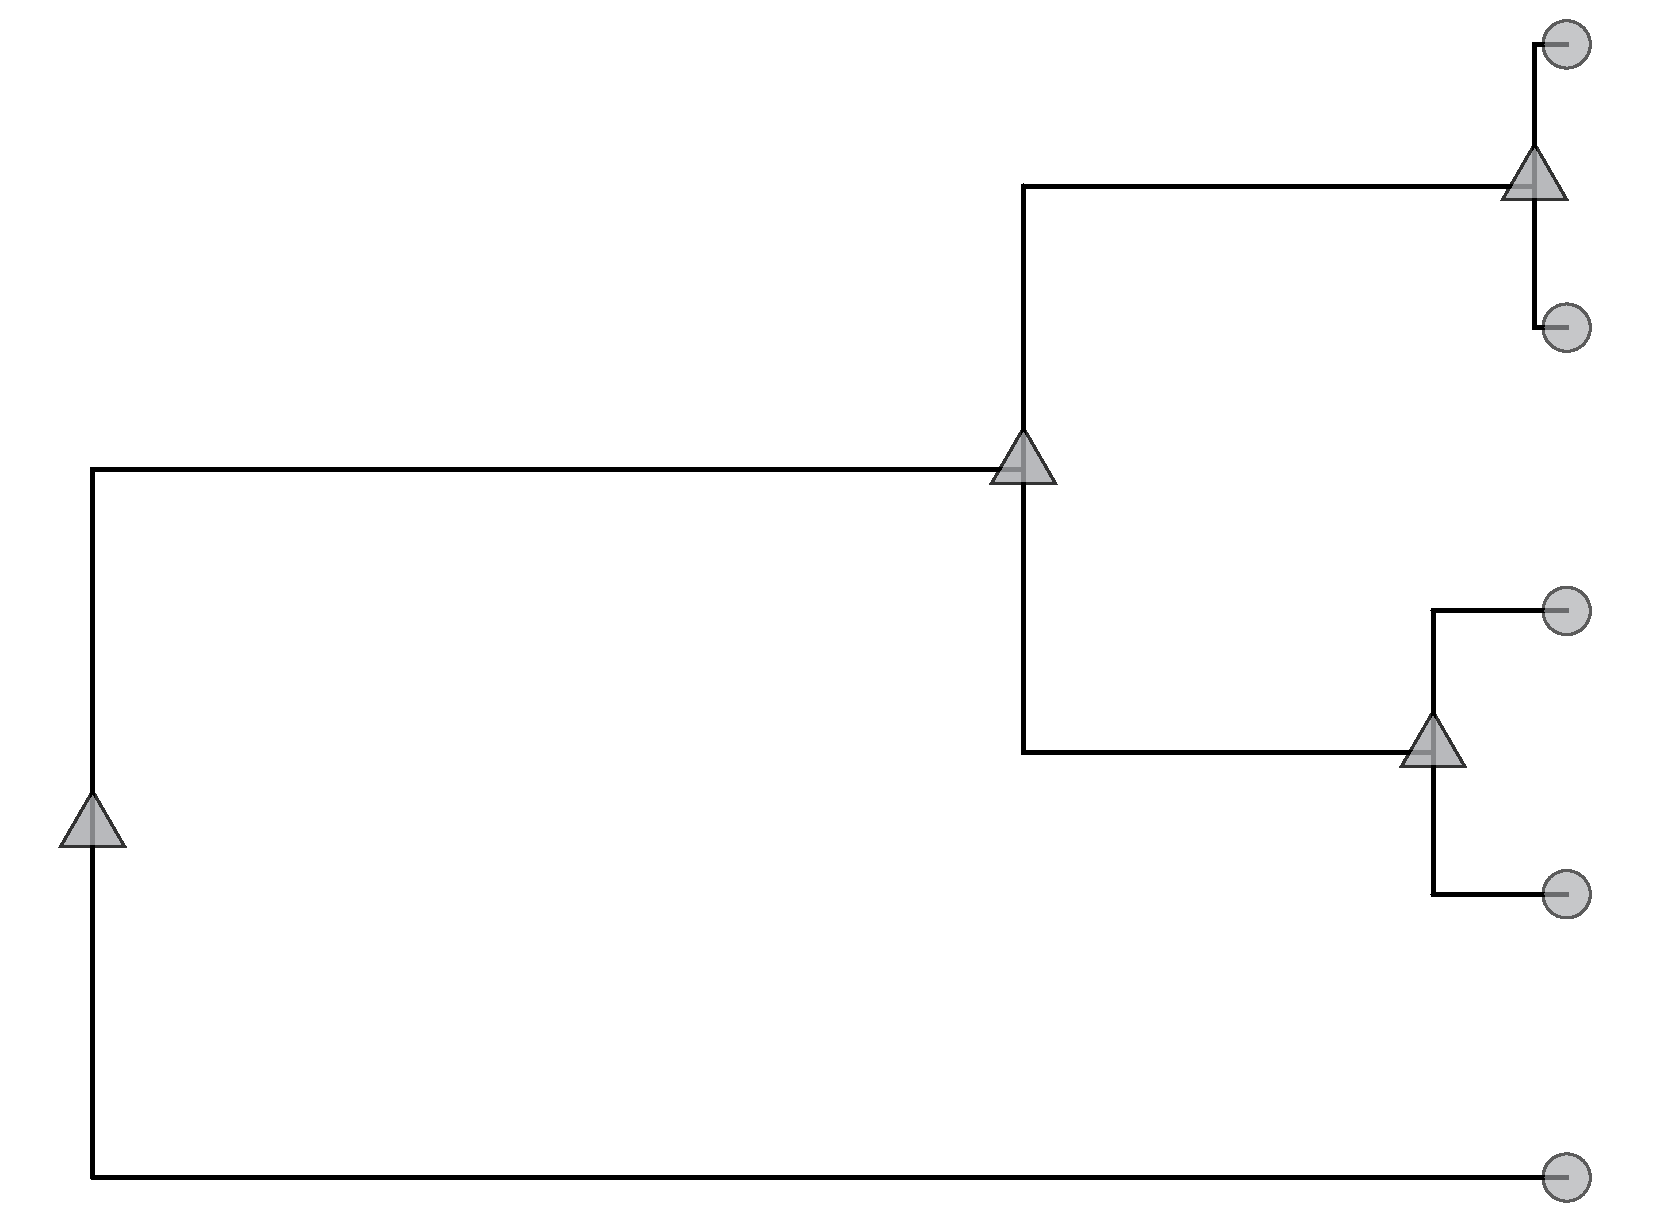
\includegraphics[height=6cm, width=7.75cm]{figures/UnscaledTree.pdf} 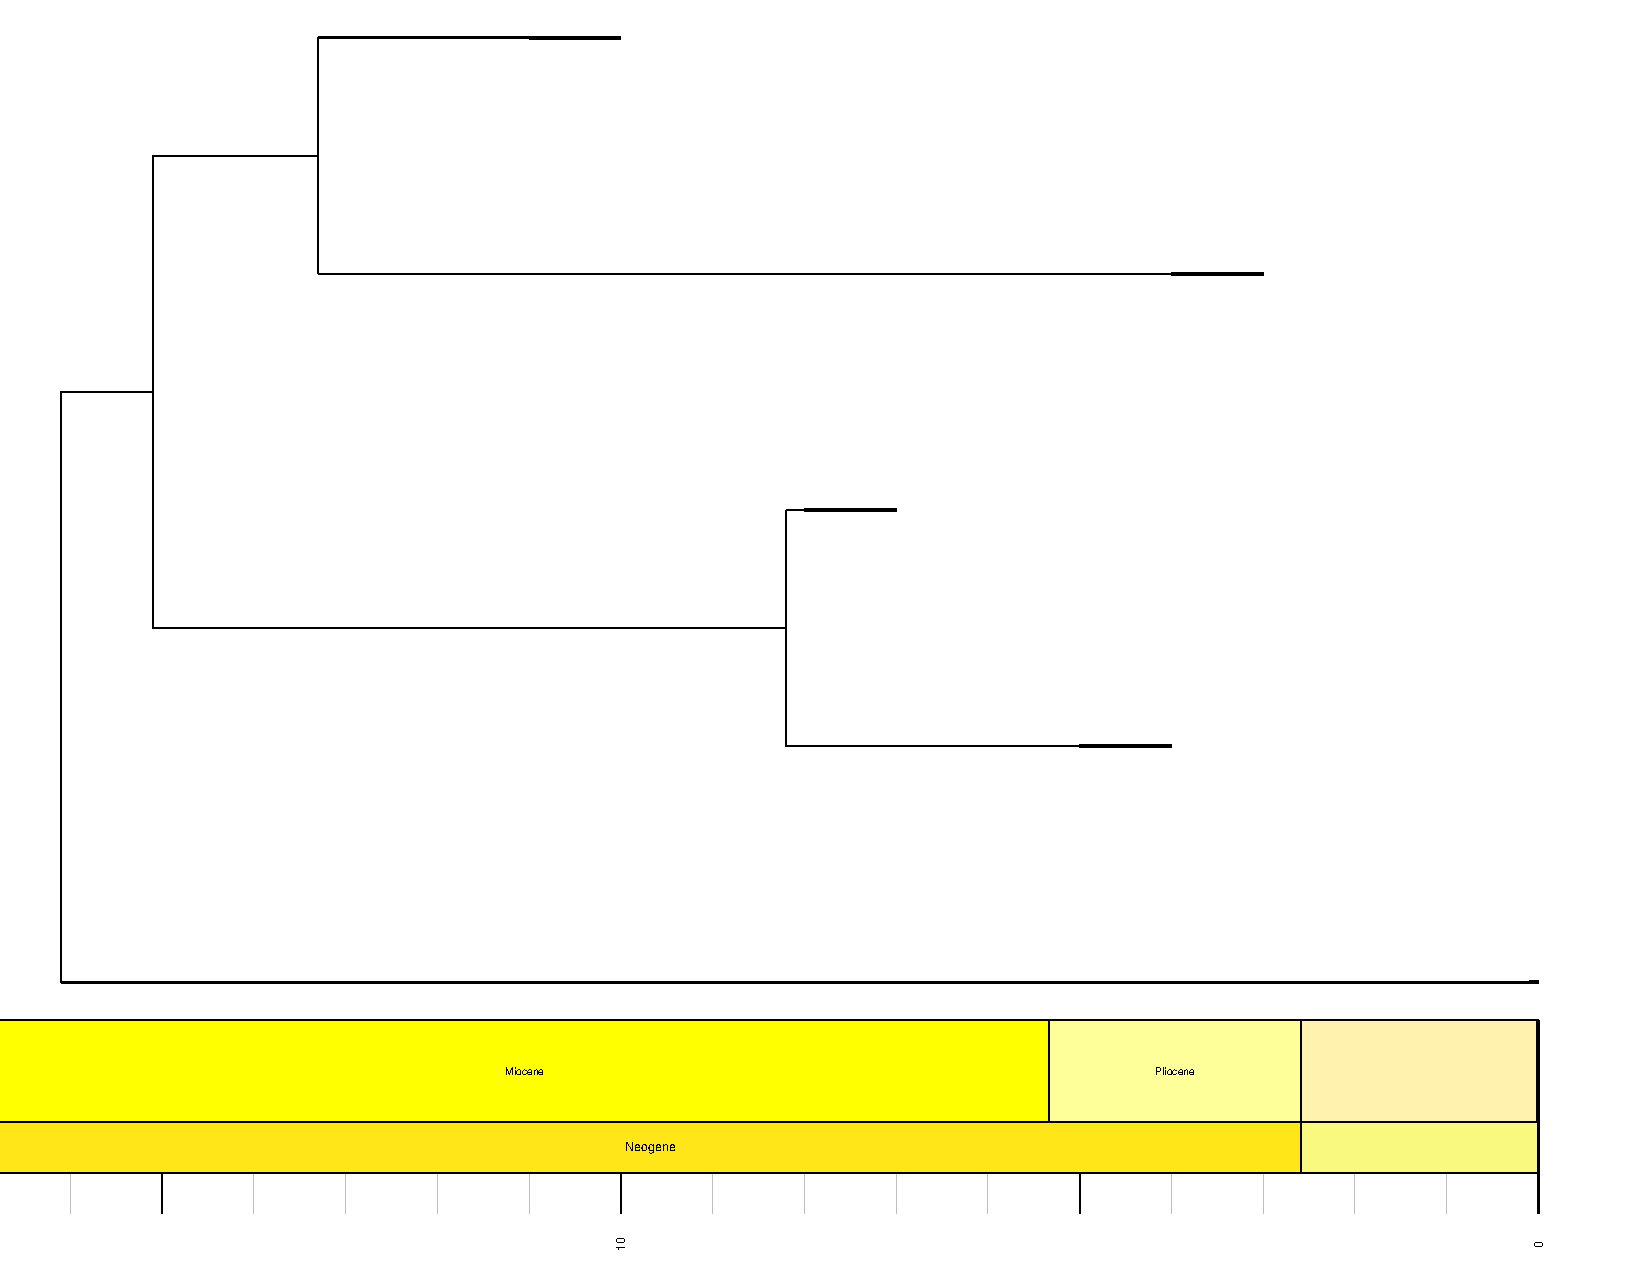
\includegraphics[height=6cm, width=7.75cm]{figures/Scaley.pdf}
\label{fig:undated}

\caption{\textbf{Undated versus dated phylogenetic inference.}
A phylogenetic tree is comprised of \textit{tips} (indicated with circles in panel A), which represent the taxa between which we aim to infer the evolutionary relationships.
These taxa are connected by \textit{branches}. %of expected character changes per character. %Under parsimony, the branch lengths may be in units of observed parsimony steps on the branch. Branches can also be referred to as \textit{edges}. 
The branches are connected by \textit{nodes} (indicated with triangles in panel A), which reflect the most recent common ancestor between two given tips. 
%You may also see nodes in the literature referred to as \textit{vertices}. \rw{I've never heard this term...}
The overall structure of the tree used to represent phylogenetic relationships is referred to as the \textit{topology}.
In an undated phylogeny branch lengths are typically in units that represent the overall amount of character change.
A tree estimated with no temporal information can be seen in panel A.
In a time calibrated tree %that has been estimated with divergence dating methods, 
the branch lengths will be in units of calendar time, often in years or millions of years. %That is, rather than reflecting an expected rate of character changes per character in the matrix, they will reflect time
Panel B shows the same tree from panel A, but with branches in millions of years.}
\label{fig:undated}

\end{figure}

\clearpage

\begin{boxedtext}{The likelihood, the prior, and the posterior}

It can be confusing for novices to understand what the likelihood, the prior, the posterior truly mean.
In plain language, the likelihood is the probability of the data given a model.
Without a model, there can be no calculation of the likelihood.

Priors can be set on parameters in the model, specifying distributions from which the value is thought to be drawn.
These distributions are often based on the researcher's intuition, and on information from prior studies.
The posterior distribution is a set of plausible solutions given the likelihood and the prior.
During Bayesian estimation, different values will be sampled for model parameters.
Their probability will be evaluated according to the likelihood and the prior.
Therefore, the posterior is proportional to the likelihood and the prior.
A good solution will often appear in the posterior sample many times.

In phylogenetics, we often refer to our models as continuous-time Markov chains.
`Continuous-time' refers to models allowing change between character states to occur instantaneously at any point in an evolutionary history.
Changes in the character state is not confined to the node; instead, branch lengths on a phylogeny are proportional to the number of expected changes per character along that particular branch. 
In this context, `Markov chain' refers to the  joint probability distribution including all the parameters for the model of morphological substitution, the model of molecular substitution, and the tree and clock models. 
In practice, this is the computer model that we use to estimate the posterior \cite{Hoehna2016b}.
\end{boxedtext}

\begin{figure}
\centering
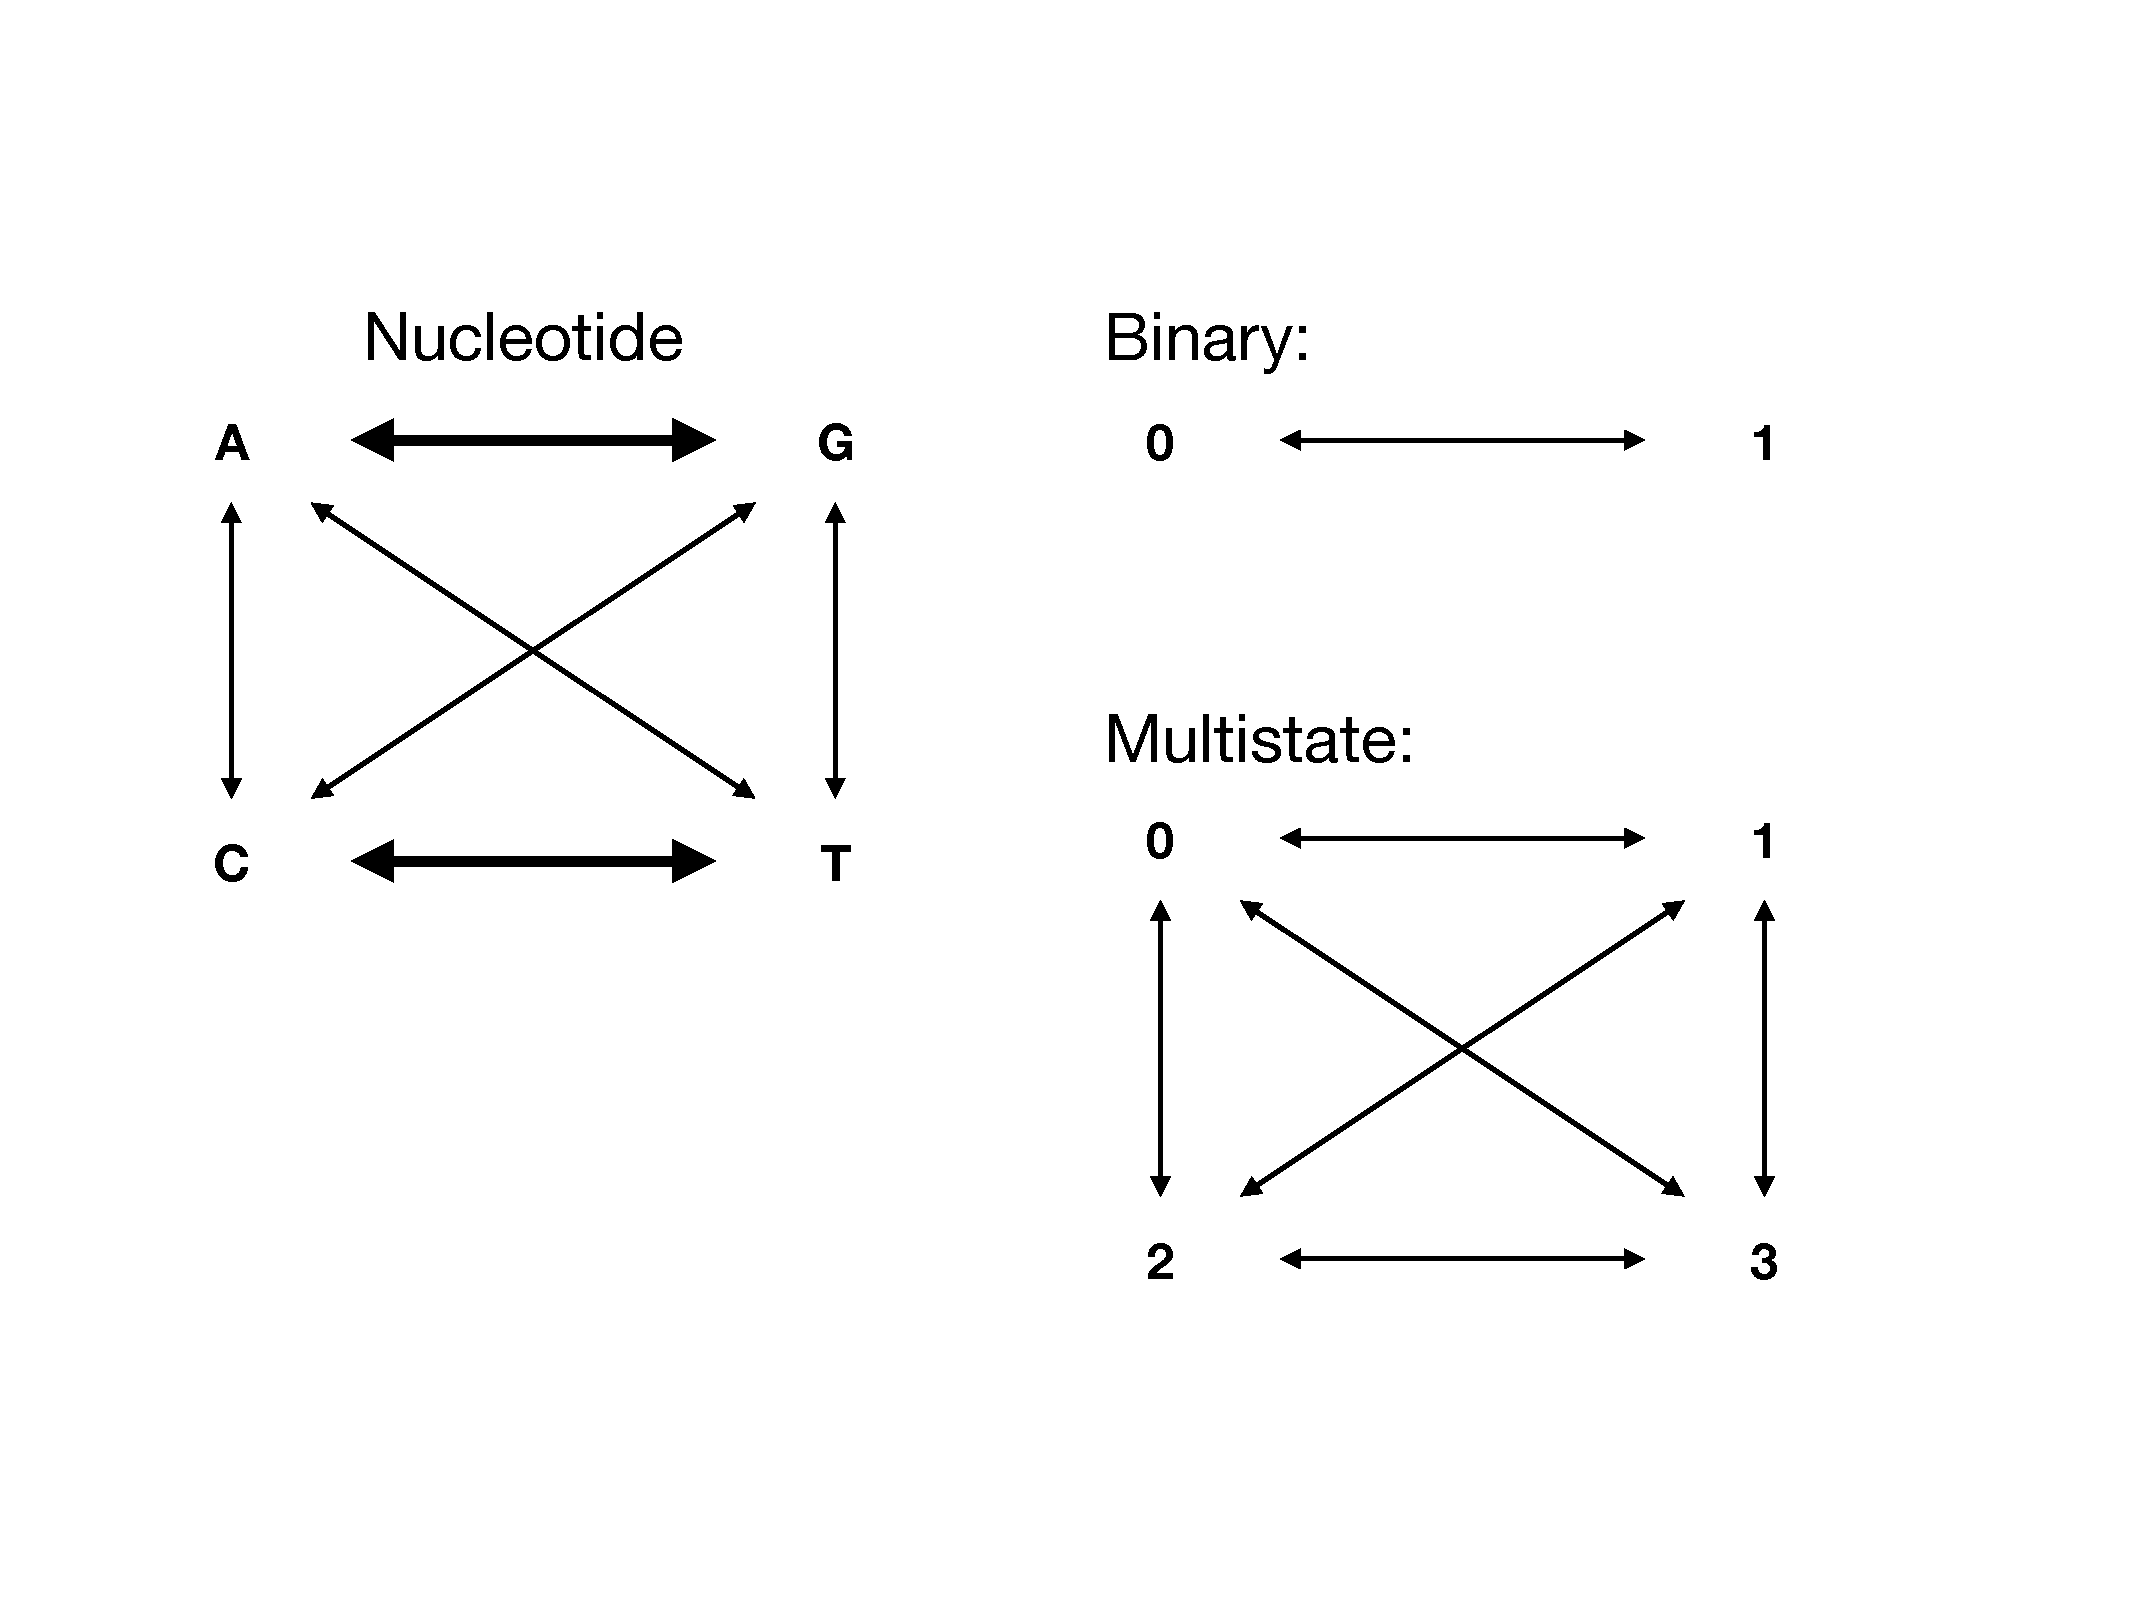
\includegraphics[width=\textwidth]{figures/Q.pdf}
\caption{\textbf{Phylogenetic $Q$ matrices.}
In this schematic, we have several representations of different types of character change.
For nucleotide data, we know that we are more likely to see certain types of change, such as two-ringed bases (purines) transitioning to other two-ringed bases, and one-ringed bases transitioning to other one-ringed bases.
This is represented by thicker arrows connecting these bases.
On the other hand, for morphological data, character states do not carry common meaning across characters.
At one character, changing, for example, from a `0' state to a `1' state may be a small change.
At another, it may mean gaining a complex character.
Therefore, researchers have largely used the Mk model of Lewis (2001) to model these data.
The schematic below shows the assumption of equal change probability between states.
}
\label{fig:Q}
\end{figure}



\begin{figure}
\centering
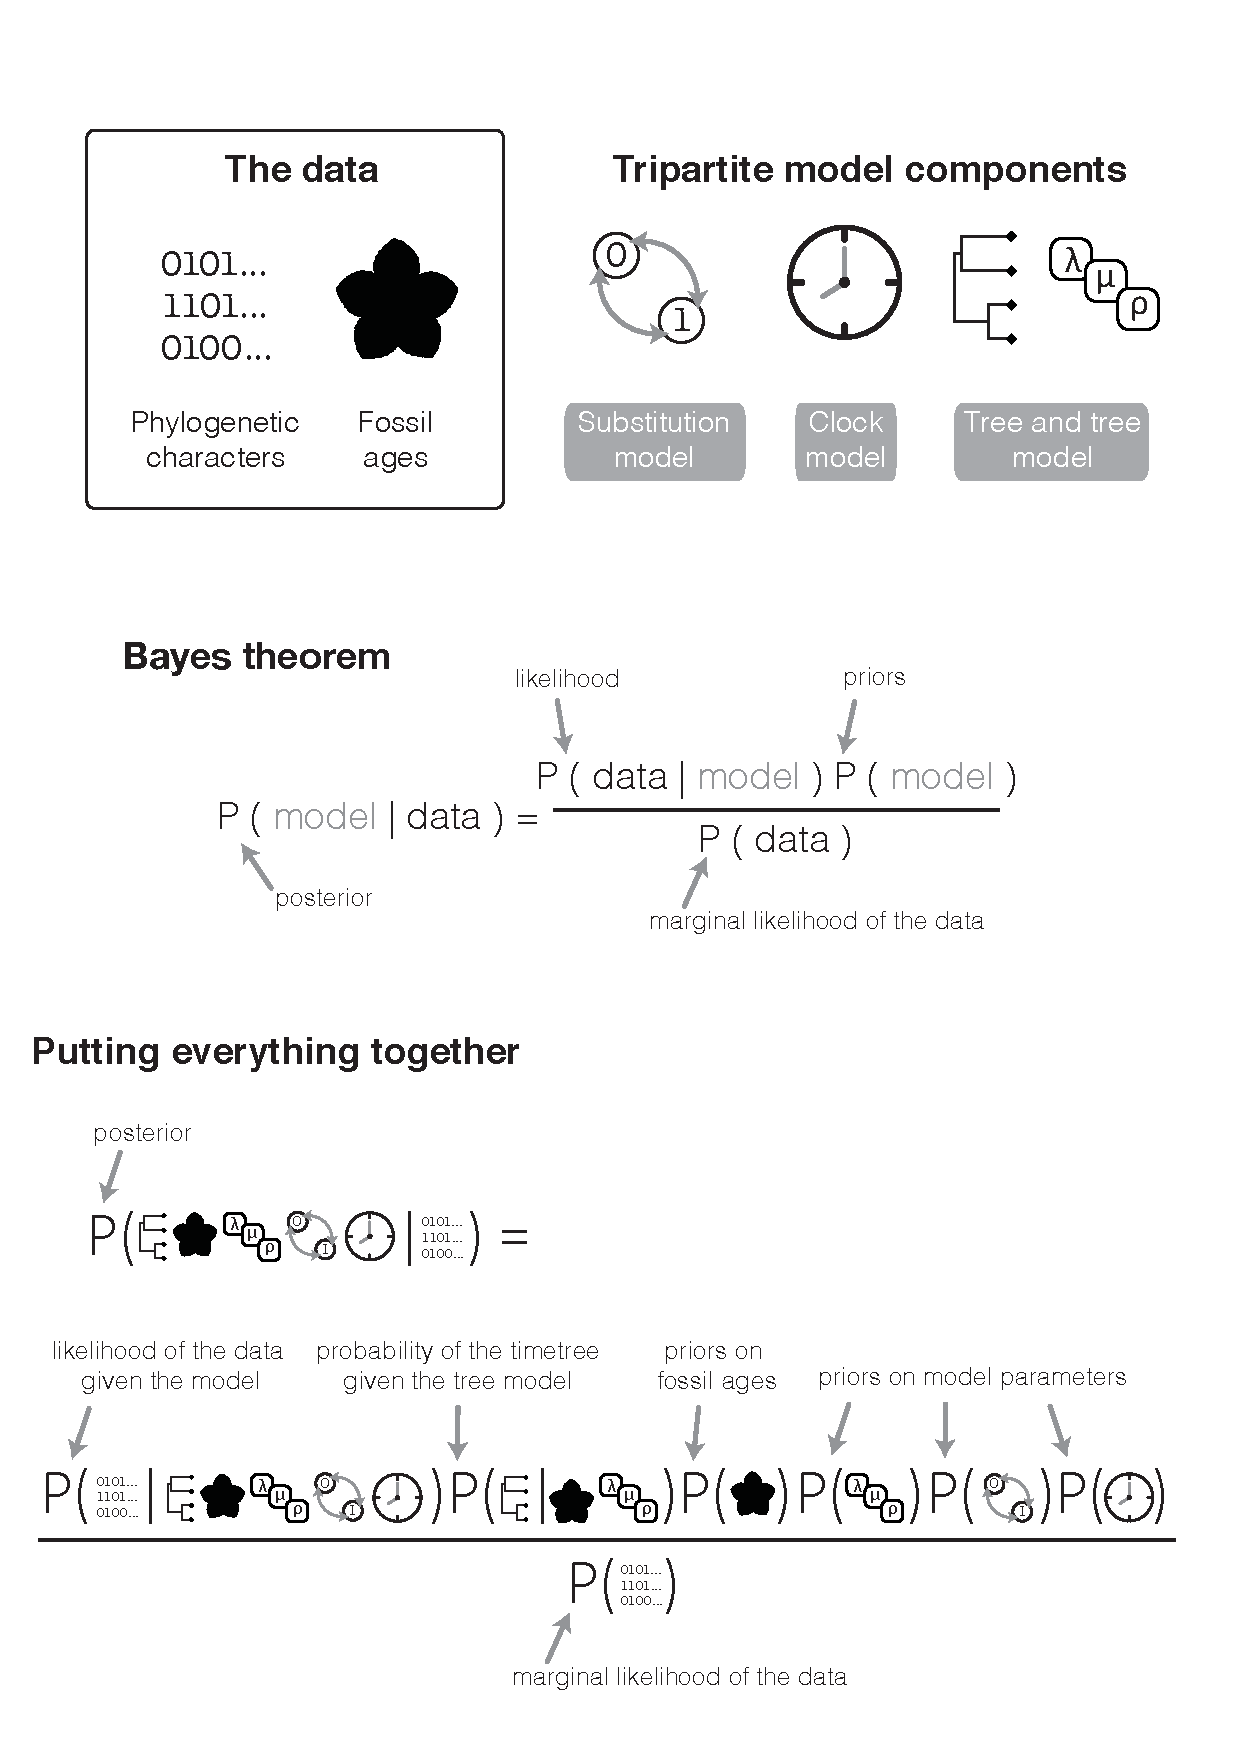
\includegraphics[width=\textwidth]{figures/bayes-theorem-v2.pdf}
\caption{\footnotesize See following page for figure legend.}
\label{fig:bayes}
\end{figure}

\clearpage

\caption{\footnotesize \textbf{A tripartite model for Bayesian divergence time estimation.}
The top panel shows the key ingredients required during inference.
The data used to generate time calibrated trees: molecular or morphological phylogenetic characters, and age information, typically fossil sampling times.
The model includes the substitution (site) model, which describes the evolution of characters, the clock model, which describes the distribution of evolutionary rates across the tree, and the tree model, which describes the distribution of speciation events across the tree.
Bayes theorem is presented in the middle panel. 
The bottom panel illustrates how everything comes together for the Bayesian estimation of divergence times.
}

\clearpage


\begin{boxedtext}{Hierarchical Models}

The tripartite approach to divergence time estimation is what is termed a \textit{hierarchical model}. 
%This is a somewhat confusing term. 
Hierarchical models are models in which variation may be described by different submodels.
In the case of divergence time estimation, the character data is described by one model, such as the Mk model.
The distribution of evolutionary rates across branches is described by the clock model.
Finally, the distribution of speciation, extinction and fossil sampling is described by the tree model.
Together, these three components are used to estimate a tree, branch lengths in units of time, and other relevant model paramters.

This term may be confusing, as model components may have a hierarchy of priors. 
For eample, if we placed a lognormal distribution with shape parameter 10 on the mean clock rate, this is a prior.
If instead, we placed an exponential prior on the shape parameter, that exponential prior is called \textit{hyperprior}.
This, while a hierarchy of priors, is not a hierarchical model. 

\end{boxedtext}
\clearpage


\begin{figure}
\centering
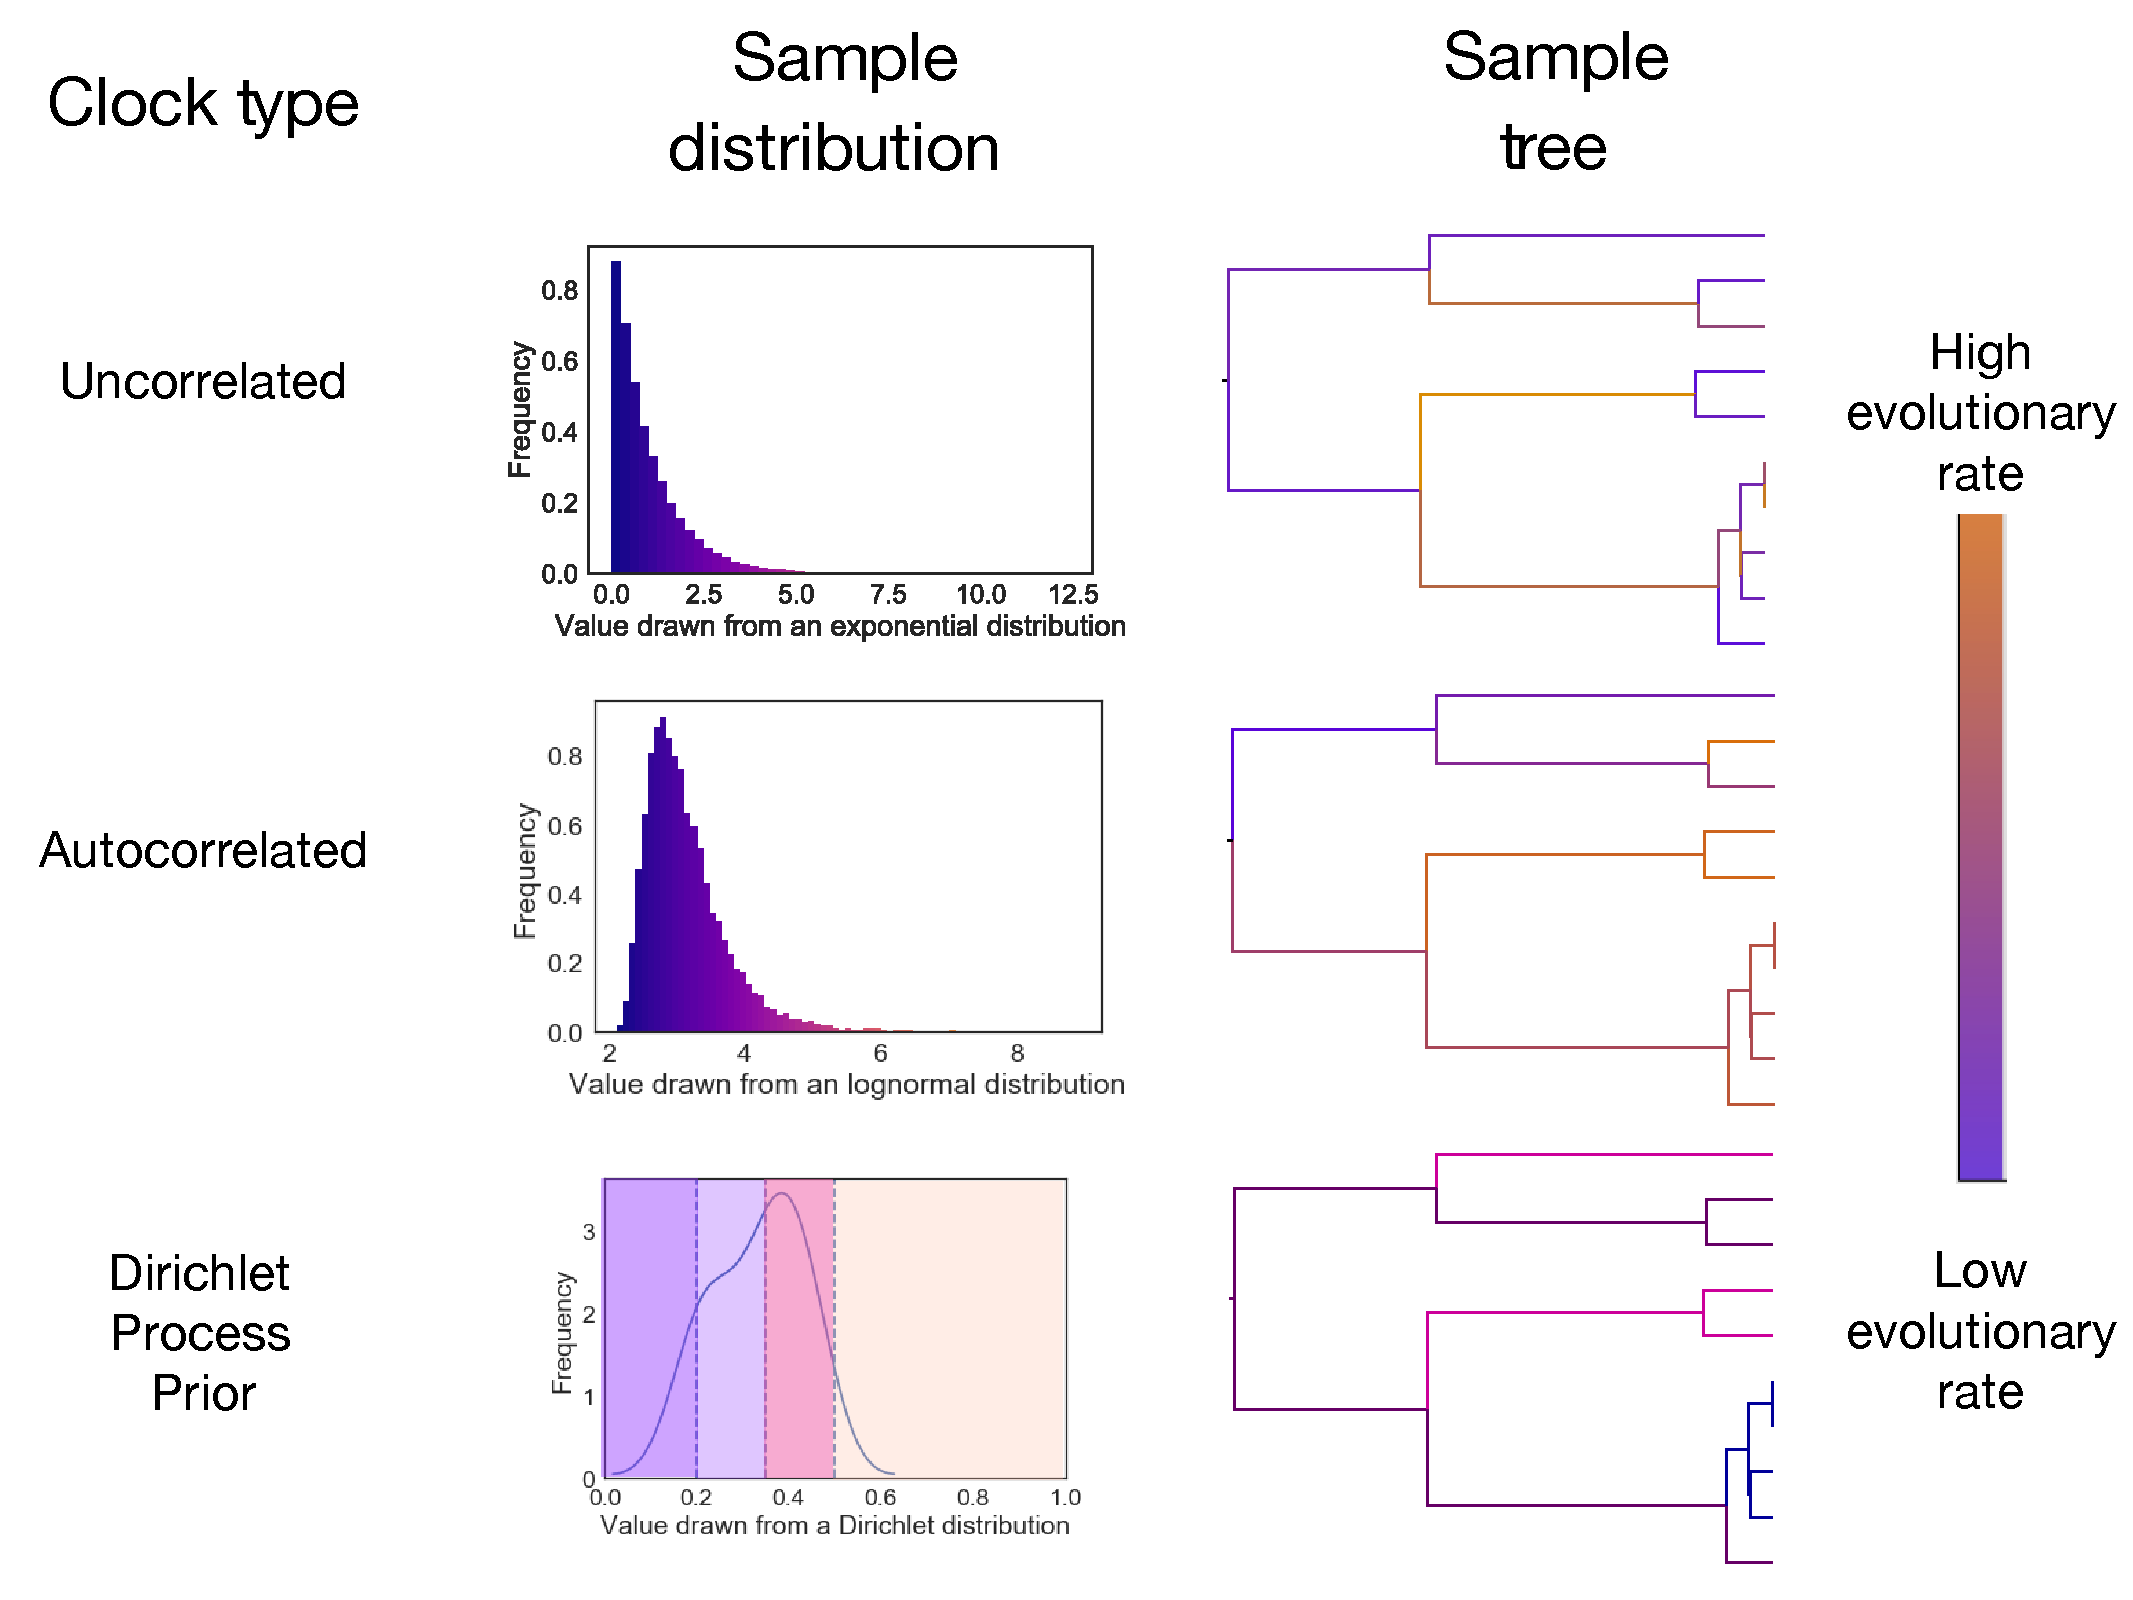
\includegraphics[width=\textwidth]{figures/Distributions.pdf}
\caption{\footnotesize See following page for figure legend.
}
\label{fig:distn}
\end{figure}

\caption{\footnotesize A schematic showing different clock models, and what they mean for the distribution of evolutionary rates across the tree. Row one shows an uncorrelated clock, with branch rates drawn from the exponential distribution. Because this clock is uncorrelated, a descendent may have a very different rate of evolution than its ancestor. In the second row, an autocorrelated clock, rates of evolution in the ancestor and descendant are expected to be more similar. The third row shows Dirichlet-distributed rates. This is a biologically agnostic clustering method for assigning branch rates.
}

\clearpage


\begin{figure}
\centering
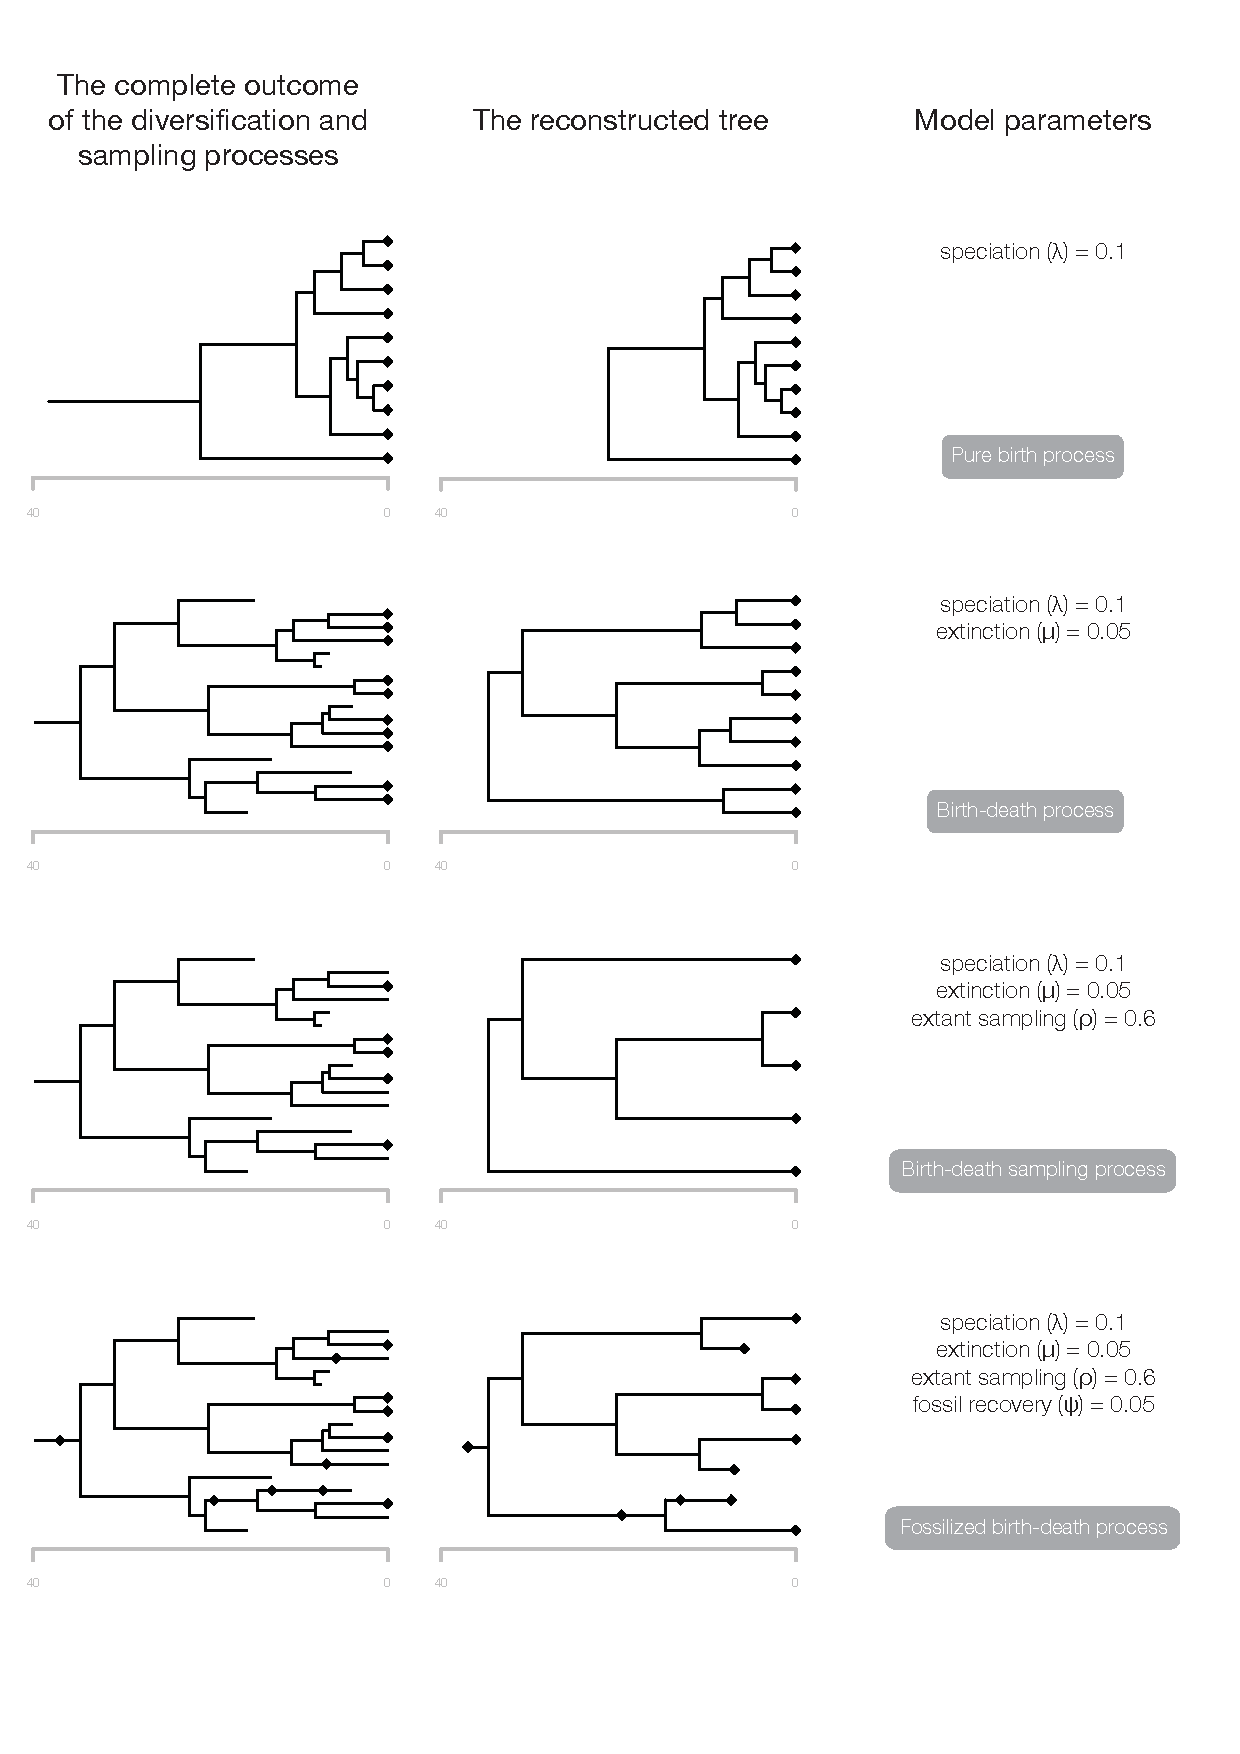
\includegraphics[width=\textwidth]{figures/birth-death-trees-v2.pdf}
\caption{\footnotesize See following page for figure legend.
}
\label{fig:birth-death}
\end{figure}

\clearpage


Figure \ref{fig:birth-death} \textbf{The complete versus reconstructed trees under birth-death process models.}
The assumptions of four different models are captured in each row.
The first column shows an example outcome of the joint diversification and sampling processes (i.e. the complete tree), where diamonds represent  extant or fossil samples.
The second column shows the tree that contains sampled lineages only (i.e. the reconstructed tree). 
The third column shows the parameters and the name commonly applied to model used to described the probability of observing the reconstructed tree shown in column two given we assume the generating processes shown in column one.
In all cases we assume constant speciation, extinction and fossil recovery, and uniform extant species sampling.
Trees and fossils were simulated and plotted using the R packages \texttt{TreeSim} \cite{Stadler2011} and \texttt{FossilSim} \cite{BaridoSottani2019b}.

\clearpage

\begin{boxedtext}{Maximum Likelihood and Bayesian Estimation}


As discussed in the section `The Likelihood', the probability of the data is calculated given a model. 
In maximum likelihood estimation, models are proposed, and the likelihood of the data is calculated given each of those models.
The model that gives the best likelihood is considered to be the `best'.
This is generally a point estimate returning one tree, one set of branch lengths, and one set of other model parameters.

Inference of undated trees from morphological data can be accomplished in many pieces of maximum likelihood software, such as PAUP \citep{Swofford2003}, RAxML \citep{Stamatakis2014}, IQTREE \citep{IQtree}, and GARLI \cite{zwickl2006}.
Estimation of dated trees incorporating morphological data has mostly been accomplished in a Bayesian context, using software such as MrBayes \cite{Huelsenbeck2002, Ronquist2003}, BEAST \citep{BEAST}, BEAST2 \citep{BEAST2} , MCMCTree \citep{MCMCtree}, and RevBayes \citep{Hoehna2014b, Hoehna2016b}.
While there is no reason models such as the FBD cannot be estimated using maximum likelihood, in practice, it is not straightforward to incorporate the uncertainty associated with parameters within a maximum likelihood framework.
\end{boxedtext}

\bibliographystyle{unsrt}
\bibliography{refs}

\end{document}

